% !TeX root = ../thuthesis-example.tex

\chapter{Structure-based Method}

\section{Introduction}

So far in the literature, no model have been using protein structural information for predicting the Michaelis
constant. However, it is known that the protein structure, also known as the terciary structure of a protein - in
opposition to the protein sequence which is known to be the primary structure of a protein - is essential. Indeed,
even though the sequence contains all the necessary information for a protein expression, many models cannot
extract all the necessary meaningful information from the primary structure and require more information. This is
where the protein structure can improve the predictions. 

Many research efforts have been put into predicting the structure of proteins such as AlphaFold or ESMFold and
these structure can be use down the line for concrete applications such as the acceleration of design 
of a drug to treat hepatocellular carcinoma (HCC), the most common type of primary liver cancer (https://www.artsci.utoronto.ca/news/new-study-uses-alphafold-and-ai-accelerate-design-novel-drug-liver-cancer)
Since the release of the AlphaFold database that contains over 200 millions structures, these methods have multiplied.
However, so far they haven't been used for predicting the Michaelis constant and our work is, to our knowledge, 
the first one to explore the use of protein structure for $K_m$ prediction.

In this chapter, we present StuctKm, a deep learning model that makes use of the protein structures of the
AlphaFold database. This method does not require any pretraining, making it fast and easily trainable. 

While the global results only outperform one out of our four benchmark models, it shows better performance 
than the current best model on the most important subset: cold proteins and cold substrates.

\section{Methods}

We now describe our data preprocessing step, input representation, model achitecture, training details, and results. 
Figure \ref{fig:seqkm} provides an overview of our method.

\begin{figure}
  \centering
  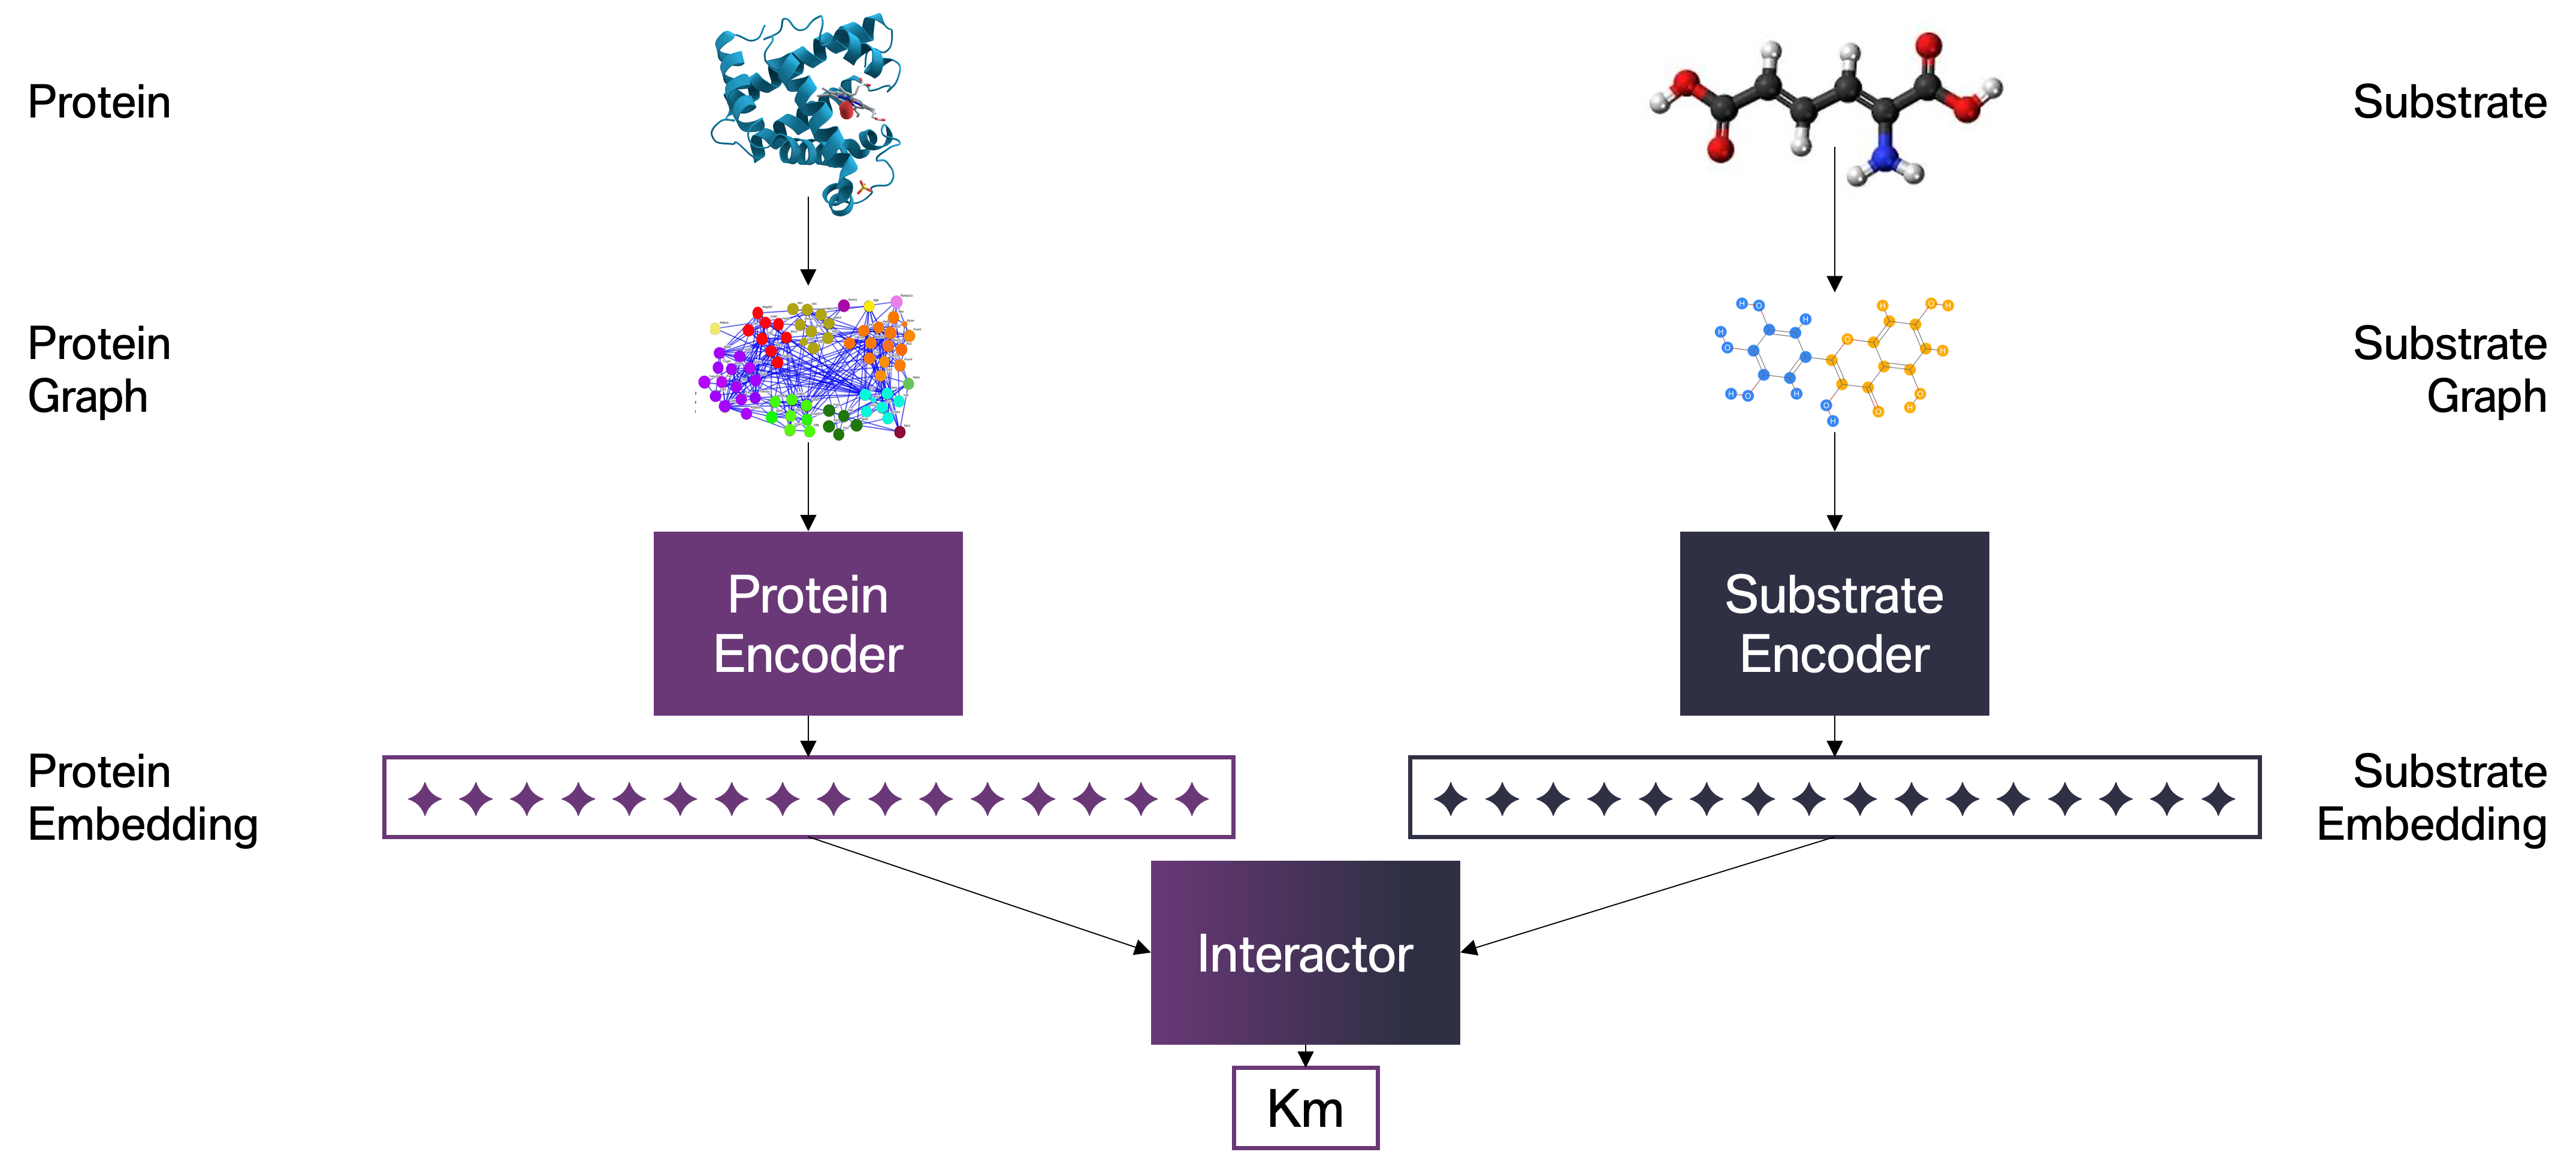
\includegraphics[width=1\linewidth]{3-structure_architecture.png}
  \caption{Overview of StructKm}
  \label{fig:structkm}
\end{figure}

\subsection{Data Preprocessing}

While the sequences were already present in the $K_m$ dataset, the structures were not. It was therefore necessary
for us to retrive them in order to use them for our structure-based model. To do so, we followed these steps:
\begin{enumerate}
  \item Identify the UniProtID of each sequence of our dataset. If it doesn't exist, find the UniProtID with the 
  highest sequence similarity rate.
  \item Download the PDB file from the AlphaFold database.
\end{enumerate}

\subsubsection{Retriving UniProtIDs}
First, we need to retrive the UniProtIDs of all the sequences of our dataset. The reason behind this is that
AlphaFold contains almost all the structure of the UniProt database, making it easy to obtain the structure.
Indeed, using only the sequence as a tool to find the relevant structure in the AlphaFold database led to finding
less than 50\% of the structures for our sequences.

The Universal Protein Resource (UniProt) is a comprehensive resource for protein sequence and annotation. The 
UniProt database is composed of the UniProt Knowledgebase (UniProtKB), the UniProt Reference Clusters (UniRef), 
and the UniProt Archive (UniParc). Specifically, UniProtKB is a comprehensive resource for protein sequence 
and annotation data. It consists of two sections: UniProtKB/Swiss-Prot and UniProtKB/TrEMBL. 
UniProtKB/Swiss-Prot provides manually annotated records with information verified by experts, 
focusing on accuracy and reliability. These annotations include function descriptions, 
domain structure, post-translational modifications, variants, and many other biological insights. 
UniProtKB/TrEMBL, on the other hand, contains automatically annotated records that have not yet been 
reviewed by humans. In this work, we will only use UniProtKB/Swiss-Prot.

To identify the UniProtID related to our protein sequences, we used a bioinformatics program called 
Basic Local Alignment Search Tool (BLAST). It can be used for comparing protein or nucleotides to sequence databases.
Specifically, we used blastp that is designed for proteins only and we compared our sequences to the 
UniProtKB/Swiss-Prot database. 

For 80\% of our sequences, we found an above 100\% sequence similarity, indicating a perfect match between our
sequence and the sequence in the UniProtKB/Swiss-Prot dataset. For the 20\% remaining, the sequence similarity is
still relatively high (above 90\% for a large proportion), indicating a high similarity. Even though the match is
not perfect, we will use these UniProtIDs and related structures and will detail in the discussion section their
impact on the results.

\subsubsection{Downloading the PDB files}

Second, once all the UniprotIDs of our sequences have been retrieved, we can download their PDB files.

A Protein Data Bank (PDB) file is a text file that contains the three-dimensional structures of molecules like
proteins and nuclic acids. These files include atomic coordinates, secondary structure assignments, 
and atomic connectivity, among other experimental metadata. The PDB format is a legacy file format that 
has been succeeded by the mmCIF format, but it is still widely used and supported by many molecular 
visualization software applications and will be used in this work.

The AlphaFold database offers all the structures predicted by the AlphaFold 2 model in PDB and mmCIF formats. 
We therefore downloaded all the structures of our UniProtIDs. 

\textbf{Note:} While UniprotIDs are unique, they might refer to the same sequences. This means that one sequence can have
several UniProtIDs. However, in the AlphaFold database, for most of the data, the structure was only generated 
for one of these UniProtIDs. Hence, before downloading the structure, we added a step to make sure to have 
the UniprotID related to the structure in the AlphaFold database.

\subsection{Input representation}

Let a protein structure be defined as a tuple $P = (S, \Sigma, \Theta, \Phi)$ where:


\begin{itemize}
  \item $P=a_1a_2a_3...a_n$ is the primary structure, a sequence of amino acids where each 
  $a_i \in A$ for $i \in \{1,..,n\}$, and $A=\{A,C,D,E,F,G,H,I,K,L,M,N,P,Q,R,S,T,V,W,Y,X\}$ is the set of 
  standard amino acids including an unknown amino acid $X$.
  \item $\Sigma = {\sigma_1, \sigma_2, ..., \sigma_m}$ represents the secondary structure, a set of 
  local structures commonly found in proteins, such as alpha helices ($\alpha$-helices) and 
  beta strands ($\beta$-strands), where each $\sigma_j$ is a tuple $(type, start, end)$ 
  with $type \in {\alpha, \beta}$ indicating the type of secondary structure, and $start, end \in \{1,..,n\}$ 
  defining the positions in the primary sequence $P$ where the structure begins and ends.
  \item $\Theta = {\theta_1, \theta_2, ..., \theta_n}$ where each $\theta_i$ corresponds to an amino acid 
  in the protein and is defined as a tuple $\theta_i = (a_i, A_i)$. $a_i \in A$ denotes the type of amino acid for 
  the $i^{th}$ position in the protein sequence. $A_i = {(\alpha_{ij}, x_{ij}, y_{ij}, z_{ij})}_{j=1}^{M_i}$ 
  represents the set of atoms for the $i^{th}$ amino acid, where $\alpha{ij}$ is the atom type 
  (e.g., carbon, nitrogen, oxygen), and $(x_{ij}, y_{ij}, z_{ij})$ are the spatial coordinates of 
  the $\alpha_{ij}$ atom in three-dimensional space. $M_i$ is the total number of atoms 
  in the $i^{th}$ amino acid.
  \item $\Phi = \{S_1, S_2, ..., S_k\}$ represents the quaternary structure, a set of protein subunits where 
  each $S_i$ is a tertiary structure, indicating how multiple polypeptide chains (subunits) 
  assemble into a functional protein complex.
\end{itemize}

Our goal is to make use of the protein as a PDB file and no longer rely on only its primary structure but 
also its terciary structure. To do so, we will use a graph representation of a protein. Each amino acid will
be represented as a node and the edges between the nodes will depends on the distance to the nodes. If the
alpha-carbons of two amino acids are less than 6 {\AA} away, then there will be an edge between them. 
If they are apart of more than 6 {\AA}, then they will not be connected. Later on, we will use Graph Neural Networks
and the message-passing paradigm that allows use to connect and allow interactions between amino acids that
might be far from each other in the protein sequence but close in its three-dimensional structure, hence making 
use of the structural information.

Furthermore, we will use the ESM2 model to generate the embeddings of the nodes of our protein graph. As the nodes
of our protein graph represent amino acids, we can use ESM2 to generate the embedding vector for each amino acid
of the sequence, that we then feed to the relevant node. This allows to add sequential information to our graph.

At the end, we obtain a protein graph with amino acids as nodes and the ESM2 embedding and the edges depending on
the structural proximity of the amino acids. We can then feed these graphs to a GNN.

For the substrate, we will once again use the Morgan Fingerprints as they represent the substrates in a way 
that can easily be used for computational tasks.

We know have two inputs that can be processed by a machine learning model.

\subsection{Model Architecture}

Similarly to our sequence-based model, our structure-based model is composed of three modules: a protein encoder 
that encode the protein, a substrate encoder that encode the substrate, and an interactor that makes the 
encoded protein and the encoded substrate interact. The main difference lies in the protein encoder.

The protein encoder is a Graph Neural Network and specifically a Graph Convolutional Neural Network (GCN). We also 
tried a Graph Attention Neural Network (GAN) and obtain similar results so we will focus here on the GCN. Our GCN
has 2 graph convolution layers that allow message passing between the nodes by aggregating neighborhood 
information. The first convolution layer is followed by a ReLU activation and a dropout layer to enhance 
feature representations while preventing overfitting. A subsequent graph convolution layer further refines 
these features, which are then globally aggregated to yield a singular, graph-level output. This output of size 128
encapsulates the structural and feature-based information of the entire graph and is one of the two inputs of 
our interactor. 

The substrate encoder is similar to the sequence-based model, the only difference being that the Morgan Fingerprints
is now a vector of size 128 and not 1024, to be consistent with the size of the protein embedding.

Finally, the interactor is a multilayer perceptron of 2 dense layers of size 256 and 128. It takes as input the
concatenated protein embedding and substrate embedding and pass it through these 2 layers to finally output a single
value, the Michaelis constant $K_m$.

\subsection{Training details}

We trained and validated our results on the same dataset we used for the sequence-based model. The only difference
being that the sequences are replaced by protein graphs. The prediction to make however is exactly the same and 
therefore the exact same methodology can be used for evaluation.

Once again, we trained our model over 300 epochs using the Adam optimizer with $\beta_1=0.9$ and $\beta_2=0.999$, and an initial
learning rate of $5\times10^{-4}$. The learning rate follows a cosine schedule, including a warmup phase of 200
steps to gradually increaser the learning rate from zero to the initial set value, ehnancing the model's convergence
stability. Training and validation batch sizes are set to 256 and 32 per device, respectively, to efficiently
utilize computational resources while maintaining an appropriate balance between speed and memory usage. 

Additionally, we leverage a cosine learning rate scheduler to adjust the learning rate dynamically, 
encouraging better fine-tuning and generalization as training progresses. To monitor the model's performance 
and ensure robustness, we log metrics every 20 steps and save the model's state every 500 steps. 
Evaluation is conducted at each step, allowing for continuous monitoring of the model's effectiveness on 
validation data. 

Finally, after looking at the best metrics for the validation test, we reverted to the saved model of the
 22nd epoch. 

 \section{Results}

 Using the model and the training strategy presented above, we obtain a MSE of 0.712 and a $r^2$ of 0.485 
 as well as the following hot/cold results for the test set:

 \begin{table}[ht]
  \centering
  \begin{tabular}{lcccccc}
  \hline
   & \multicolumn{3}{c}{\textbf{Hot}} & \multicolumn{3}{c}{\textbf{Cold}} \\
   & Samples & MSE & R\(^2\) & Samples & MSE & R\(^2\) \\ \hline
  \textbf{Hot seq}  & 1135 & 0.644 & 0.485 & 64 & 0.795 & 0.475 \\
  \textbf{Cold seq} & 1042 & 0.746 & 0.505 & 98 & 1.066 & 0.135 \\ \hline
  \end{tabular}
  \caption{StructKm results on the test set}
  \label{tab:summary_performance}
\end{table}

For the new test set, we obtain a total MSE of 1.257 and a total $r^2$ of 0.286. In details:

\begin{table}[ht]
  \centering
  \begin{tabular}{lcccccc}
  \hline
   & \multicolumn{3}{c}{\textbf{Hot}} & \multicolumn{3}{c}{\textbf{Cold}} \\
   & Samples & MSE & R\(^2\) & Samples & MSE & R\(^2\) \\ \hline
  \textbf{Hot seq}  & 40 & 1.439 & 0.067 & 30 & 0.827 & -0.190 \\
  \textbf{Cold seq} & 1117 & 1.175 & 0.306 & 102 & 2.202 & -0.078 \\ \hline
  \end{tabular}
  \caption{StructKm results on the new test set}
  \label{tab:summary_performance}
\end{table}

The lower results for the new test set are due to a low similarity (34\%) similarity for the UniProtID 
matches with the sequence using BLAST for this set. Hence, the structures do not accurately represent the
proteins, introducing noise into the data and lowering the performances.

Overall, our method offer better performances only for 1 out of the 4 models of our benchmark, which indicates 
possible improvements. However, we also notice the 0.135 for the cold proteins and cold substrates, which is
one of the most important of our work as our goal is to find new possible drugs and hence it must be a cold protein
and a cold substrate. This value is above the 0.11 of ProSmith and is extremely important for our work. We will
discuss it in more details in the discussion part.

\section{Pocket Detection Model}

In this section, we present an alternative to the structure-based model. So far, we have always presented
a model using the entire protein. However, as we explained it in Section \textcolor{red}{literature review},
the reaction between the enzyme and the substrate operate in a specific part of the protein which is called
a pocket. Hence, we believe that if we can efficiently find the pocket for each protein and use it instead of
the entire sequence, we may obtain better results and reduce the noise inputed by parts of the protein that 
are not relevant for predicting the Michaelis constant. 

To do, different methods can be used and we will focus on fpocket. fpocket is an open-source command line
tool designed for the identification and analysis of protein pockets. It is widely used in computational
biology as it predicts potential binding sites on the surface of protein structures and do so very quickly
compared to other more novel and more computaionally expensive deep learning methods for pocket detection.

We therefore used fpocket to identify the best pockets for each of our protein structure, selected the top
one pocket, and then took the subgraph
corresponding to this predicted pocket and used it as an input in our structure-based model. The subgraph 
being a graph, the model didn't required any modification. With a similar methodoly than previously, we
trained our model and obtained an MSE of 0.770 and a correlation coefficient of 0.443. Specifically,
we have:

\begin{table}[ht]
  \centering
  \begin{tabular}{lcccccc}
  \hline
   & \multicolumn{3}{c}{\textbf{Hot}} & \multicolumn{3}{c}{\textbf{Cold}} \\
   & Samples & MSE & R\(^2\) & Samples & MSE & R\(^2\) \\ \hline
  \textbf{Hot seq}  & 1192 & 0.672 & 0.461 & 64 & 0.934 & 0.373 \\
  \textbf{Cold seq} & 985 & 0.823 & 0.461 & 98 & 1.324 & -0.063 \\ \hline
  \end{tabular}
  \caption{SeqKm results on the test set}
  \label{tab:results_pocket_test}
 \end{table}

For the new test set, we have an MSE of 1.233 and a correlation coefficient of 0.300. Specifically,

\begin{table}[ht]
  \centering
  \begin{tabular}{lcccccc}
  \hline
   & \multicolumn{3}{c}{\textbf{Hot}} & \multicolumn{3}{c}{\textbf{Cold}} \\
   & Samples & MSE & R\(^2\) & Samples & MSE & R\(^2\) \\ \hline
  \textbf{Hot seq}  & 40 & 1.322 & 0.114 & 30 & 0.873 & -0.289 \\
  \textbf{Cold seq}& 1117 & 1.166 & 0.312 & 102 & 2.033 & 0.010 \\ \hline
  \end{tabular}
  \caption{SeqKm results on the test set}
  \label{tab:results_pocket_new_test}
 \end{table}

As we observed, our results for the pocket model are lower than for the full protein. To understand why in
details, we made an analysis on the pockets we found, the main goal being to determine if the pockets we found
were actual pockets. This task is difficult as our protein structure are generated by AlphaFold and hence do
not contain any annotations about the real pocket where the enzymatic reaction happens. However, some of the
proteins possess experimentally determined crystallographic structures where the pocket is anotated. From 
these, we can have a better understanding of our model and its capabilities.

Hence for all the protein which had a known crystallographic structure, we retrieved them from the Protein 
Data Bank and run the fpocket algorithm on top of it to verify if the real pocket where indeed at the 
locations predicted by the algorithm. We manage to retrieve around 2,000 real structures which is about 
20\% of our dataset. While it is only a subset of our dataset, we should still be able to obtain meaningful
insights that may explain the lower performance.

Running the fpocket algorithm on these crystallographic structures, we obtain the following results:
\begin{itemize}
  \item Top 1: 55.17\%
  \item Top 3: 69.62\%
  \item Top 5: 72.96\%
\end{itemize}
This means that half of the time, the pocket we detect with fpocket and that we use in our downstream application
is not the real pocket. Hence our training data includes some incorrect data which seems to explain why
our model is performing more poorly using pockets that the entire structure.

While the idea of using the local information (pocket) instead of the global information (full structure)
seems very interesting and makes biological sense, it does not seems to be possible using only the best pocket
predicted by fpocket. 
Using the top 3 or top 5 pockets may be useful but would need a tailored approach to feed these pockets to
the model.
It could also be possible to use different models for pockets detection but we decided to not continue in this 
direction as we believe that decent results can be obtained by using the global information only, as described
in the following chapter.